\section{A Practical Approach to the Simulation of Safety-critical Automotive Control Systems considering Complex Data Flows}

\subsection*{overview}
\begin{itemize}
	\item Issue of determining end to end latencies in systems composed of functional and dysfunctional modes of operations.
	\item Depending on required safety level the complexity of implementation varies.
	\item Development consists of finding the real time bottlenecks, verifying and deploying, and as such is complex.
	\item Aims to provide virtual integration of system early in development stages.
\end{itemize}
\subsection*{Main points}
\begin{itemize}
	\item Important task is planning execution of tasks and ISRs.
	\item Model based simulation of various execution scenarios to determine the worst case overhead of task executions.
	\item Event chain used to specify a sequence of execution and data flow, subject to RT requirement.
	\begin{minipage}{\linewidth}
		\centering
		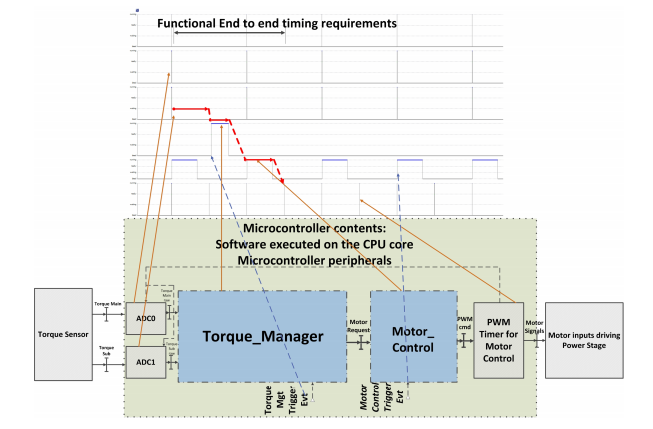
\includegraphics[width=13cm]{Pictures/Event-chain.png}
	\end{minipage}
	\item Initially data flow between hardware and software components at system level were modeled using flow port concept of \textit{SysML}.
	\item Formalized model analyzed using INCRON tool-suite for:
	\begin{itemize}
		\item Deadline Violation.
		\item End to End latency.
		\item Start to Start jitter.
		\item CPU peak load in certain averaging intervals.
		\item Response time distribution.
	\end{itemize}
	\item Aspects of system configuration to be considered for optimizing event chains:
	\begin{itemize}
		\item Periods of the time-triggered tasks.
		\item Number and decomposition of the processes.
		\item Execution order.
		\item Core affinity.
	\end{itemize}
	\item Iterative design flow defined. Consists of:
	\begin{itemize}
		\item Specify structural system architecture.
		\item Identify interaction between application and basic software.
		\item Specify the dynamic system architecture comprising of tasks and their basic timing properties.
		\item Specify functional data and control flow.
		\item Perform safety analysis and identify dysfunctional control flow for all relevant faults.
		\item Define, Create and run simulation on timing analysis tool like chronSIM.
		\item Extract timing properties and define the architecture. 
	\end{itemize}
\end{itemize}
\subsection*{Reference}
https://hal.archives-ouvertes.fr/hal-01291352/document